%\documentclass[twocolumn]{article}
\documentclass{article}
\usepackage[english]{babel}
\usepackage[a4paper,left=15mm,top=15mm,right=15mm,bottom=15mm]{geometry}

%multi column line 

\usepackage{makecell}  % Add this to your preamble

%\usepackage{natbib}
\usepackage{graphicx}
\bibliographystyle{plainnat}
%\usepackage{booktabs, tabularx}
\usepackage{multicol}
\usepackage{comment}

\usepackage{caption}
\usepackage{subcaption}
\usepackage{float}

% Reference
\usepackage[backend=biber, style=numeric]{biblatex}
\addbibresource{references.bib}
\usepackage{hyperref}  % This makes links clickable.

% Column related
%\setlength{\parindent}{1pt} % Adjusts the indentation at the start of a new paragraph.
%\setlength{\parskip}{5pt} % Adjusts vertical space between paragraphs.

%\usepackage[title]{appendix}

\title{
\includegraphics{images/0.ITU-logo.png}\\[1cm] \huge{Research Project}\\
    \begin{center}
    \line(1,0){250}
    \end{center}
    \huge{Decision Tree and Convolutional Neural Network Models for Audio Feature Classification in Depression Prediction}
    \begin{center}
    \line(1,0){250}
    \end{center}
    }
\author{
  Gergo Gyori  (gegy@itu.dk) \\
  Supervised by: Stella Graßhof (stgr@itu.dk) 
}
\date{2024-12-16}

\begin{document}

\maketitle

\begin{abstract}
This study explores the utility of vocal biomarkers for depression diagnosis through binary classification methods. Using audio features extracted from speech in the DAIC-WOZ and EATD-Corpus datasets, I employ decision tree algorithms and other machine learning models to evaluate their predictive accuracy. These methods demonstrate considerable promise for clinical application, underlining both the precision and practicability of vocal biomarkers in mental health diagnostics. The findings confirm the effectiveness of audio-based features in depression screening and discuss the broader implications for future psychiatric assessment tools, potentially revolutionizing approaches to mental health diagnostics.
\end{abstract}


% multicolum version 2
\begin{multicols}{2}

\bigskip % Adds vertical space
\noindent\textbf{Keywords:} depression detection \textbullet{} audio analysis \textbullet{} machine learning \textbullet{} CNN \textbullet{} MFCC

\section{Introduction}
%\subsection{Background and Motivation}
Depression is a significant global health concern affecting millions of people worldwide.\cite{WHO_Mental_Disorders_2019} Early detection and intervention are crucial for effective treatment. Traditional methods of depression assessment rely heavily on clinical interviews and self-reported questionnaires, This research explores the potential of automated depression detection through audio analysis, leveraging machine learning techniques to identify patterns in speech that may indicate depressive states.

In this paper I have used EATD-Corpus\cite{shen2022automaticdepressiondetectionemotional} and Distress Analysis Interview Corpus - Wizard of Oz
(DAIC-WOZ)\cite{Gratch2014}\cite{DAICWOZ}

%\subsection{Problem Statement}
The challenge lies in accurately detecting depression from audio features while handling:
\begin{itemize}
    \item Class imbalance in depression severity categories
    \item Complex relationship between audio characteristics and mental state
    \item Need for interpretable results for clinical applications
\end{itemize}
\section{Datasets Description}
\subsection{DAIC}
The Distress Analysis Interview Corpus - Wizard of Oz (DAIC) \cite{DAICWOZ} dataset is a valuable resource for developing algorithms to diagnose conditions like depression and anxiety. It consists of 189 interview sessions conducted in English with an animated virtual agent named Ellie in a simulated clinical environment. This dataset includes audio recordings, text transcripts, and annotations for verbal and non-verbal cues, such as facial expressions through Action Units \cite{AU}.

Participants were assessed using the PHQ-8 depression screening tool, derived from a self-reported survey. The PHQ-8 scores, with 10 or higher indicating depression, are the outcome of these surveys. The dataset is structured into three subsets to maintain data integrity: 107 participants in the training set, 35 in the development set, and 47 in the test set.

The dataset is particularly suited for analyzing vocal characteristics, speech patterns, and non-verbal behaviors associated with mental health states. Its detailed annotations support advanced studies into multimodal integration techniques, enhancing AI-driven mental health assessments.

In my research, I will focus exclusively on the audio data to explore vocal characteristics related to mental health. 

\subsection{EATD}
The Emotional Audio-Textual Depression Corpus \cite{shen2022automaticdepressiondetectionemotional} dataset includes audio recordings and their corresponding textual transcripts from interviews conducted with both depressed and non-depressed volunteers. Each participant has six audio recordings—two each of neutral, positive, and negative sentences—in both cleaned and original formats.

The EATD is distinctive as it is the first publicly available Chinese dataset that integrates both audio and text modalities specifically for depression analysis. It comprises contributions from 162 student volunteers. Each session in the dataset is annotated according to the Self-Rating Depression Scale (SDS) \cite{SDS}.

% This corpus not only enriches the tools available to researchers but also supports the development of sophisticated, accessible, and non-invasive diagnostic and treatment tools for mental health, aligning with the broader goals of improving mental health care through technology.
\section{Literature Review}
During the literature review, I primarily focused on the DAIC dataset for several reasons. Firstly, while the EATD dataset is relevant, it is considerably smaller in scale, containing only three single sentences (negative, positive, neutral) from 162 participants. In contrast, the DAIC dataset provides a more comprehensive array of audio and textual data from 189 participants, enhancing the potential to train more robust machine learning models. This choice allows for a deeper exploration of methodologies and outcomes pertinent to the use of vocal biomarkers in depression detection within a larger and more varied participant base, thereby improving the generalization and statistical power of the findings.

For finding the best accuracy, this paper\cite{liu2024diagnostic} was used, and three three papers were checked which reached the best accuracy. Among these Homsiang et al\cite{homsiang2022classification} achieved 95\% accuracy using a 1D CNN architecture with data augmentation. Their approach involved converting audio to Mel Cepstral Coefficients (MCC) and implementing various augmentation techniques including noise reduction, pitch shifting, and speed adjustment. Their comparative study of different architectures (1D CNN, 2D CNN, LSTM, and GRU) demonstrated that 1D CNN with augmented data significantly outperformed other approaches, showing strong performance in both depression detection (precision: 0.91, recall: 1.00) and non-depression classification (precision: 1.00, recall: 0.90). This work particularly highlights the importance of data augmentation in improving model performance, as their non-augmented experiments only achieved 71\% accuracy with 2D CNN.

Ishmaru et al. \cite{ishimaru2023classification} achieved 97\% accuracy using a Graph Convolutional Neural Network (GCNN) approach that analyzes correlations between audio features. Their model represented the relationships between 65 different audio features (including 24 MCC) as graph structures, allowing it to capture complex interactions between voice characteristics. They conducted two types of experiments: one with overlapping subjects in training and test sets (Setting 1, Speaker-dependent test) and another with completely separated subjects (Setting 2, Speaker-independent test). While Setting 1 achieved 95\% accuracy, Setting 2's performance dropped significantly, highlighting a critical challenge in generalizing to new patients. This finding raises important questions about the practical applicability of current depression detection models when applied to previously unseen patients. This research suggests that while high accuracies are achievable in controlled settings, real-world application requires addressing the gap between training and new patient performance.

Yin et al. \cite{yin2023depression} introduced a novel approach to depression detection from speech by combining transformers with parallel Convolutional Neural Networks (TCC), achieving an accuracy of 94\% using 40 band Mel-Frequency Cepstral Coefficients (MFCC). This method of feature extraction was critical in maintaining the fidelity of audio signals, thereby enhancing model accuracy. Importantly, the high accuracy was obtained under experimental conditions similar to "Setting 1" from prior research, where the model was trained and tested on audio samples from the same set of participants. This setup often leads to inflated performance metrics due to the model's limited generalization to new subjects. Their model, which incorporates two CNN streams for local feature extraction alongside a transformer using linear attention mechanisms with kernel functions, reduces computational demands while enhancing the ability to capture temporal dynamics in speech. The results, derived from the DAIC dataset, indicated that their hybrid model outperforms traditional CNN-LSTM architectures. This showcases the effectiveness of parallel processing and advanced attention mechanisms in recognizing depression from long speech sequences, highlighting the importance of robust feature extraction techniques like the 40 band MFCC in achieving high model performance.

In the literature on audio processing for depression detection, various audio preprocessing techniques have been utilized to enhance the quality of the data before analysis. Notably, Homsiang's approach involved some form of audio preprocessing, though specific details are not provided. Other studies have explicitly detailed their methods: for example, Ishmaru et al. described techniques for speech enhancement that include noise estimation and filtration using deep learning models, aiming to improve the clarity and quality of the audio data for better model performance\cite{kantamaneni2023speech}

Conversely, Yin et al. opted not to apply any preprocessing to their audio data. This approach can offer insights into the raw data's effectiveness but may require more sophisticated modeling techniques to deal with potential noise and variability in the audio signals.

This variety in approaches highlights a crucial aspect of audio-based depression detection research: the balance between enhancing data quality through preprocessing and developing models robust enough to handle raw, unfiltered data.
%\input{related_work}
\section{Methodology}

\subsection{Data Preparation}

PHQ8 values are organized to  multiclass\cite{kroenke2001phq}. The values are organized into binary values as well based on\cite{kroenke2009phq}. In case of EATD the SDS index the SDS index is categorized by and it is mapped to binary categories.

The table below shows the mapping of the PHQ8 values to binary values.

\begin{table}[H]
    \centering
    \begin{tabular}{|c|c|}
    \hline
    PHQ8 Value & Binary Value \\ \hline
    0-4        & 0            \\ \hline
    5-27       & 1            \\ \hline
    10-14      & 2            \\ \hline
    15-19      & 3            \\ \hline
    20-27      & 4            \\ \hline
    \end{tabular}
    \caption{Mapping
    PHQ8 values to binary values}
    \label{tab:phq8 to binary mapping}

For extrating features for the DT I have used Mel-Frequency Cepstral Coefficients (MFCCs)\cite{tiwari2010mfcc} features. 

MFCCs are pivotal for analyzing the power spectrum of audio signals, particularly in tasks like speech recognition. The extraction involves transforming the audio signal from the time domain to the frequency domain using the Fast Fourier Transform (FFT) to capture frequency components. Subsequently, these components are mapped onto the mel scale via a mel filter bank that mimics the human auditory system's response more effectively than linearly-spaced frequency bands. The outputs of the mel filter bank are logged to approximate human perception of loudness, followed by a Discrete Cosine Transform (DCT) to de-correlate the log mel spectrum, resulting in MFCCs that represent the audio signal's timbral characteristics effectively.

Additional spectral features such as centroid, bandwidth, and rolloff, alongside the zero-crossing rate and overall signal energy, are computed. These features, combined with the statistical mean and standard deviation across frames, form a comprehensive feature vector for each audio sample. This method captures not only the fundamental qualities of sound but also complex characteristics related to speech dynamics and tonal quality, rendering it suitable for emotion recognition from speech.

For the audio preparation: No additional audio  was performed on the audio files before went under the MFCC analysis. In case of the DAIC the segments where the patient speaks are cut from the audio. Each chunks is goes under the audio extraction. Later on the min, avg and max values across all chunk per each patient are extracted and used to feed the DT. For CNN the whole MFCC spectrum is used. In case of EATD: the uncloeand sentences were used for audio extraction: neutral, positive and negative, meaning 3 values where averaged, min and so on. 


% MODELS

\subsection{Models}
Two model will be built for the evaluation. One is a decission tree (DT) another one is a Transformer-CNN-CNN (TCC)\cite{yin2023depression}.

\subsection{DT}

The determination of the optimal number of features and tree depth for the Decision Tree classifier is central to enhancing model performance and mitigating overfitting. The selection of the most predictive features is facilitated by an ANOVA-based feature ranking, which identifies features that significantly contribute to model accuracy. This feature selection process is integrated with depth tuning of the Decision Tree to find the optimal combination that yields the highest accuracy on the validation set.

To address potential overfitting, we systematically explore tree depths ranging from 1 to 19, assessing the model's performance with varying numbers of top-ranked features at each depth. The evaluation metrics include F1-score and accuracy, with a particular emphasis on the weighted average F1-score due to the imbalanced nature of our dataset. This metric adjusts for label imbalance by weighting the F1-score of each class by its support (the number of true instances for each label). This approach ensures that our model's performance is robust across different class distributions and provides a more reliable indication of its generalization ability.

The final model parameters—optimal feature count and tree depth—are selected based on their performance on the development set, aiming to maximize the weighted average F1-score while maintaining generalizability across the dataset.

\subsection{TCC}

I have adapted the TCC model for our application. The model consists of two parallel CNN streams and a transformer stream, integrating both local and global information processing capabilities. In my adaptation, I employ the CNN streams to extract local features from the input while the transformer stream captures the temporal dynamics through linear attention mechanisms, optimized for the dataset.

Each CNN stream processes the input independently to capture diverse aspects of the data, and the transformer stream analyzes the sequence as a whole. The outputs of these streams are then fused, combining their feature spaces to enhance the model's prediction accuracy. This fusion happens in a fully connected layer that integrates learned features before the final classification layer.

Modifications include adjusting the dimensionality of the input features and streamlining the transformer's attention mechanism to reduce computational complexity.


\section{Experimental Setup}
\subsection{Feature Selection}

DT

For finding the best features which corrolate with the binary depression score ANOVA, Random Forest (RF) and Mutual information was used. Despite the unbalanced dataset ANOVA produced the best result. 
\subsection{Model Parameters}
\subsection{Evaluation Metrics}
\subsection{Implementation Details}
\section{Results and Analysis}


% \begin{table*}[t]
%     \centering
%     \caption{Comparison of Depression Detection Models}
%     \scalebox{0.9}{
%     \begin{tabular}{|l|l|l|c|l|l|l|}
%     \hline
%     \textbf{Author} & \textbf{Dataset} & \textbf{Model} & \textbf{F1-score (\%)} & \makecell{\textbf{Speaker} \\ \textbf{Dependency}} & \textbf{Features} & \makecell{\textbf{Additional} \\ \textbf{Features}} \\
%     \hline
%     Gergo Gyori & DAIC & DT & 65 & Independent & MFCC & No \\
%     \hline
%     Gergo Gyori & EATD & DT & 68 & Independent & MFCC & No \\
%     \hline
%     Gergo Gyori & DAIC & TCC & 74 & Dependent & MFCC & No \\
%     \hline
%     Gergo Gyori & DAIC & TCC & 58 & Dependent & MFC & No \\
%     \hline
%     Gergo Gyori & DAIC & CNN & 50 & Independent & MFCC & No \\
%     \hline
%     Ishimaru et al. & DAIC & CNN & 96 & Dependent & MFCC & Yes \\
%     \hline
%     Ishimaru et al. & DAIC & CNN & 49 & Independent & MFCC & Yes \\
%     \hline
%     Yin et al. & DAIC & TCC & 93 & Dependent & MFCC & Yes \\
%     \hline
%     Homsiang et al. & DAIC & 1D CNN & 95 & Dependent & MFC & No \\
%     \hline
%     \label{tab:model-comparison}
%     \end{tabular}
%     }
% \end{table*}


\begin{table*}[t]
    \centering
    \caption{Comparison of Depression Detection Models}
    \scalebox{0.9}{
    \begin{tabular}{|l|l|l|c|l|l|l|}
    \hline
    \textbf{Author} & \textbf{Dataset} & \textbf{Model} & \textbf{F1-score (\%)} & \makecell{\textbf{Speaker} \\ \textbf{Dependency}} & \textbf{Features} & \makecell{\textbf{Additional} \\ \textbf{Features}} \\
    \hline
    Gyori & DAIC & DT & 65 & Independent & MFCC & No \\
    \hline
    Gyori & EATD & DT & 68 & Independent & MFCC & No \\
    \hline
    Gyori & DAIC & TCC & 74 & Dependent & MFCC & No \\
    \hline
    Gyori & DAIC & TCC & 58 & Dependent & MFC & No \\
    \hline
    Gyori & DAIC & CNN & 50 & Independent & MFCC & No \\
    \hline
    Ishimaru et al. & DAIC & CNN & 96 & Dependent & MFCC & Yes \\
    \hline
    Ishimaru et al. & DAIC & CNN & 49 & Independent & MFCC & Yes \\
    \hline
    Yin et al. & DAIC & TCC & 93 & Dependent & MFCC & Yes \\
    \hline
    Homsiang et al. & DAIC & 1D CNN & 95 & Dependent & MFC & No \\
    \hline
    \end{tabular}
    }
    \label{tab:model-comparison}
\end{table*}

\subsection{Analysis of Speaker Dependency}
A critical insight emerged during the analysis of different studies' performance metrics: the distinction between speaker dependent and independent approaches significantly impacts reported results. In \textit{speaker dependent} setups, different segments from the same participant's interview can appear in both training and test sets -- for example, various 30-second chunks from a single 5-minute interview might be distributed across both sets. While this ensures no exact duplicate segments exist between sets, the model can still learn speaker-specific characteristics.

In contrast, \textit{speaker independent} approaches maintain strict separation: all segments from a participant's interview are allocated either entirely to training or test sets. This previously unaddressed factor in my methodology explains the substantial performance differences observed in Table \ref{tab:model-comparison}, where speaker dependent approaches consistently show higher F1-scores compared to speaker independent setups. This finding highlights the importance of clearly specifying speaker dependency when reporting depression detection results.

\begin{figure}[H]
    \centering
    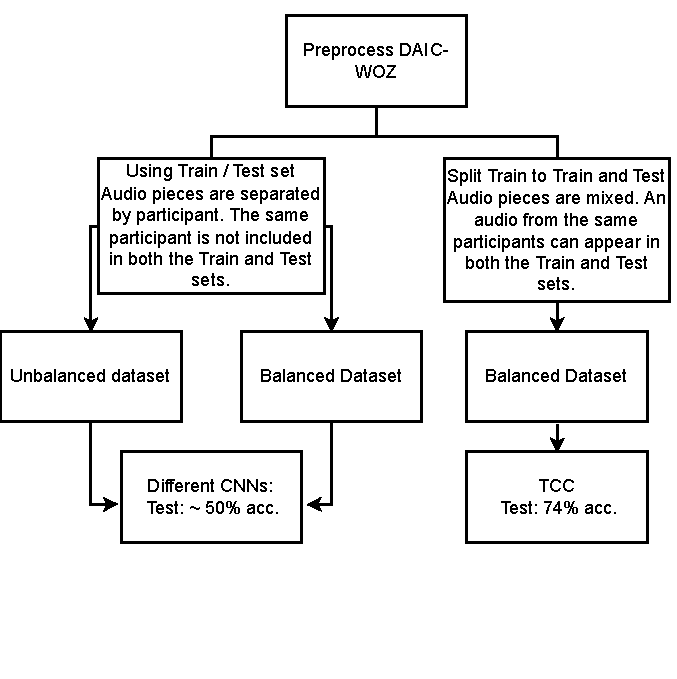
\includegraphics[width=0.45\textwidth]{vis_pdf/Train Test problem.drawio.pdf}
    \caption{Train/Test split strategies and their results (DAIC)}
    \label{fig:train_test_split_problems}
\end{figure}

This section presents the results of the experiments conducted in this study, organized into subsections focusing on specific aspects of the project. Initially, the performance of DT models is compared across the DAIC and EATD datasets. In the subsequent TCC section, only the DAIC dataset is used for evaluation. The different strategies are visualized on figure ~\ref{fig:train_test_split_problems}.




Table \ref{tab:model-comparison} provides a comparison of the models discussed in the literature, highlighting the differences in dataset, model, F1-score, split strategy, speaker dependency, features, and additional features. The models are evaluated based on their performance on the DAIC dataset, with the F1-score serving as the primary metric for comparison.



\subsection{Model Performance - DT}
While the models showcased performance on the DAIC dataset with an accuracy of 98.11\% on the training set (Tables \ref{table:classification_report_train_daic} and Figures \ref{fig:confusion_matrices_daic}, \ref{table:classification_report_dev_daic}), a significant drop in performance was observed on the development set.

Particularly, the development set for the DAIC dataset displayed only a 66\% accuracy (Table \ref{table:classification_report_dev_daic}), suggesting issues with the model's ability to generalize to new data. 

Similarly, for the EATD dataset, while the training results were promising with an accuracy of 87\% (Table \ref{table:classification_report_train_eatd}), the development set results were considerably lower, achieving only a 68\% accuracy (Table \ref{table:classification_report_dev_eatd}). This performance decrement underscores the necessity to consider alternative modeling strategies that might improve generalization across unseen datasets.


\begin{table}[H]
    \centering
    \caption{Classification Report on Training Set - DAIC}
    \scalebox{0.8}{% Scale the table to 50% of the original size
    \begin{tabular}{|c|c|c|c|c|}
    \hline
    \textbf{Class} & \textbf{Precision} & \textbf{Recall} & \textbf{F1-score} & \textbf{Support} \\ \hline
    0              & 0.97               & 1.00            & 0.99              & 76               \\ \hline
    1              & 1.00               & 0.93            & 0.97              & 30               \\ \hline
    \multicolumn{5}{|c|}{\textbf{Accuracy}: 0.98 \textbf{of} 106}                         \\ \hline
    \multicolumn{5}{|c|}{\textbf{Macro Avg}: Precision 0.99, Recall 0.97, F1-score 0.98} \\ \hline
    \multicolumn{5}{|c|}{\textbf{Weighted Avg}: Precision 0.98, Recall 0.98, F1-score 0.98} \\ \hline
    \end{tabular}}
    
    \label{table:classification_report_train_daic}
\end{table}


\begin{table}[H]
    \centering
    \caption{Classification Report on Development Set - DAIC}
    \scalebox{0.8}{% Scale the table to 50% of the original size
    \begin{tabular}{|c|c|c|c|c|}
    \hline
    \textbf{Class} & \textbf{Precision} & \textbf{Recall} & \textbf{F1-score} & \textbf{Support} \\ \hline
    0              & 0.76               & 0.65            & 0.70              & 20               \\ \hline
    1              & 0.53               & 0.67            & 0.59              & 12               \\ \hline
    \multicolumn{5}{|c|}{\textbf{Accuracy}: 0.66 \textbf{of} 32}                          \\ \hline
    \multicolumn{5}{|c|}{\textbf{Macro Avg}: Precision 0.65, Recall 0.66, F1-score 0.65} \\ \hline
    \multicolumn{5}{|c|}{\textbf{Weighted Avg}: Precision 0.68, Recall 0.66, F1-score 0.66} \\ \hline
    \end{tabular}}
    
    \label{table:classification_report_dev_daic}
\end{table}

\begin{figure}[H]
    \centering
    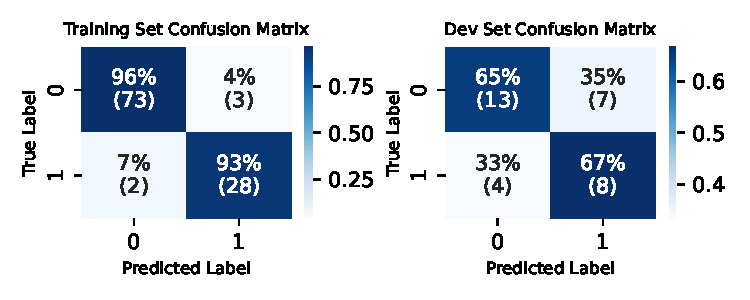
\includegraphics[width=0.45\textwidth]{vis_pdf/daic_all_confusion_matrices.pdf} % Adjust the scale to fit the page
    \caption{Confusion Matrices - DAIC}
    \label{fig:confusion_matrices_daic}
\end{figure}


%EATD

%TRAIN

\begin{table}[H]
    \centering
    \caption{Classification Report on Training Set - EATD}
    \scalebox{0.8}{% Scale the table to 80% of the original size
    \begin{tabular}{|c|c|c|c|c|}
    \hline
    \textbf{Class} & \textbf{Precision} & \textbf{Recall} & \textbf{F1-score} & \textbf{Support} \\ \hline
    0              & 0.96               & 0.84            & 0.90              & 56               \\ \hline
    1              & 0.74               & 0.93            & 0.82              & 27               \\ \hline
    \multicolumn{5}{|c|}{\textbf{Accuracy}: 0.87 \textbf{of} 83}                        \\ \hline
    \multicolumn{5}{|c|}{\textbf{Macro Avg}: Precision 0.85, Recall 0.88, F1-score 0.86} \\ \hline
    \multicolumn{5}{|c|}{\textbf{Weighted Avg}: Precision 0.89, Recall 0.87, F1-score 0.87} \\ \hline
    \end{tabular}}
    
    \label{table:classification_report_train_eatd}
\end{table}



\begin{table}[H]
    \centering
    \caption{Classification Report on Dev. Set- EATD}
    \scalebox{0.8}{% Scale the table to 80% of the original size
    \begin{tabular}{|c|c|c|c|c|}
    \hline
    \textbf{Class} & \textbf{Precision} & \textbf{Recall} & \textbf{F1-score} & \textbf{Support} \\ \hline
    0              & 0.71               & 0.88            & 0.79              & 52               \\ \hline
    1              & 0.54               & 0.27            & 0.36              & 26               \\ \hline
    \multicolumn{5}{|c|}{\textbf{Accuracy}: 0.68 \textbf{of} 78}                        \\ \hline
    \multicolumn{5}{|c|}{\textbf{Macro Avg}: Precision 0.62, Recall 0.58, F1-score 0.57} \\ \hline
    \multicolumn{5}{|c|}{\textbf{Weighted Avg}: Precision 0.65, Recall 0.68, F1-score 0.64} \\ \hline
    \end{tabular}}
    
    \label{table:classification_report_dev_eatd}
\end{table}


\begin{figure}[H]
\centering
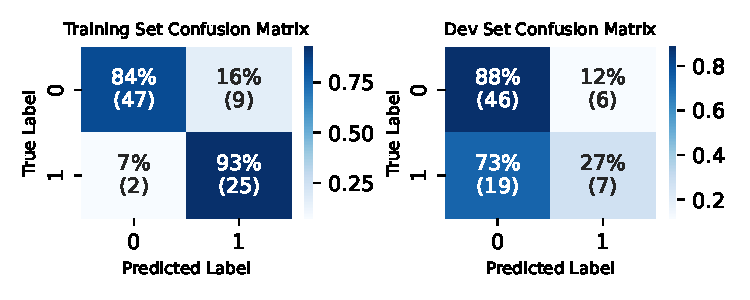
\includegraphics[width=0.45\textwidth]{vis_pdf/eatd_all_confusion_matrices.pdf} % Adjust the scale to fit the page
\caption{Confusion Matrices - EATD}
\label{fig:confusion_matrices_eatd}
\end{figure}

Training DT on both DAIC and EATD datasets revealed that ANOVA selected different top features for each dataset, indicating potential challenges in generalizing the model across different data conditions.

\subsection{Model Performance - CNN}

In my experiments with various CNN models described in the literature, the models consistently underperformed, achieving only 50\% accuracy on the development set (see Table \ref{tab:model-comparison}). A deeper investigation into the literature revealed a critical distinction: while speaker independent approaches (where participants' data is strictly separated between train and test sets) showed similar modest performance, models achieving high accuracy (>90\%) were predominantly using speaker dependent setups.

This performance gap is evident in Table \ref{tab:model-comparison}, where speaker dependent approaches by Ishimaru et al., Yin et al., and Homsiang et al. achieved F1-scores of 96\%, 93\%, and 95\% respectively, while speaker independent implementations, including our implementation, struggled to exceed 50\%. In speaker dependent setups, different segments from the same participant's interview were distributed between train and test sets, allowing models to learn individual speech characteristics rather than generalizable depression indicators.

The CNN models struggled to generalize when tasked with predicting new, unseen participants. The variance in accuracy across different CNN architectures is not discussed in this report. Instead, we focus on the results from the TCC model, detailed in Figure \ref{fig:confusion_matrices_TCC_daic}.
The training and validation accuracy and loss are depicted in Figure \ref{fig:training_TCC_daic}. The model underwent training for approximately 100 epochs, not to achieve the best possible accuracy but to demonstrate the model’s learning capability.
The model reached a 74\% accuracy on the development set, using a lightweight version of the architecture proposed by Yin et al \cite{yin2023depression}. The evaluation metrics presented are based on the model's performance at its peak accuracy.

\begin{figure}[H]
    \centering
    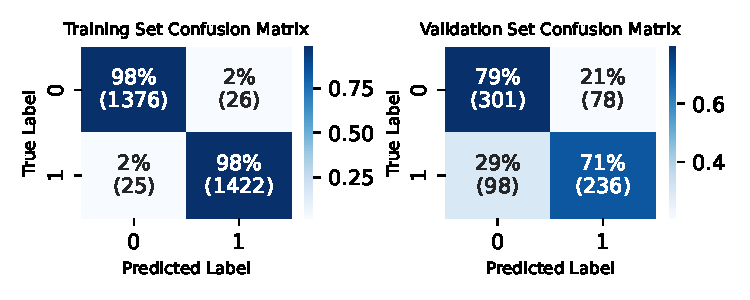
\includegraphics[width=0.45\textwidth]{vis_pdf/TCC_FINAL.pdf} % Adjust the scale to fit the page
    \caption{Confusion Matrices (Speaker Dependent - DAIC)}
    \label{fig:confusion_matrices_TCC_daic}
\end{figure}

\begin{figure}[H]
    \centering
    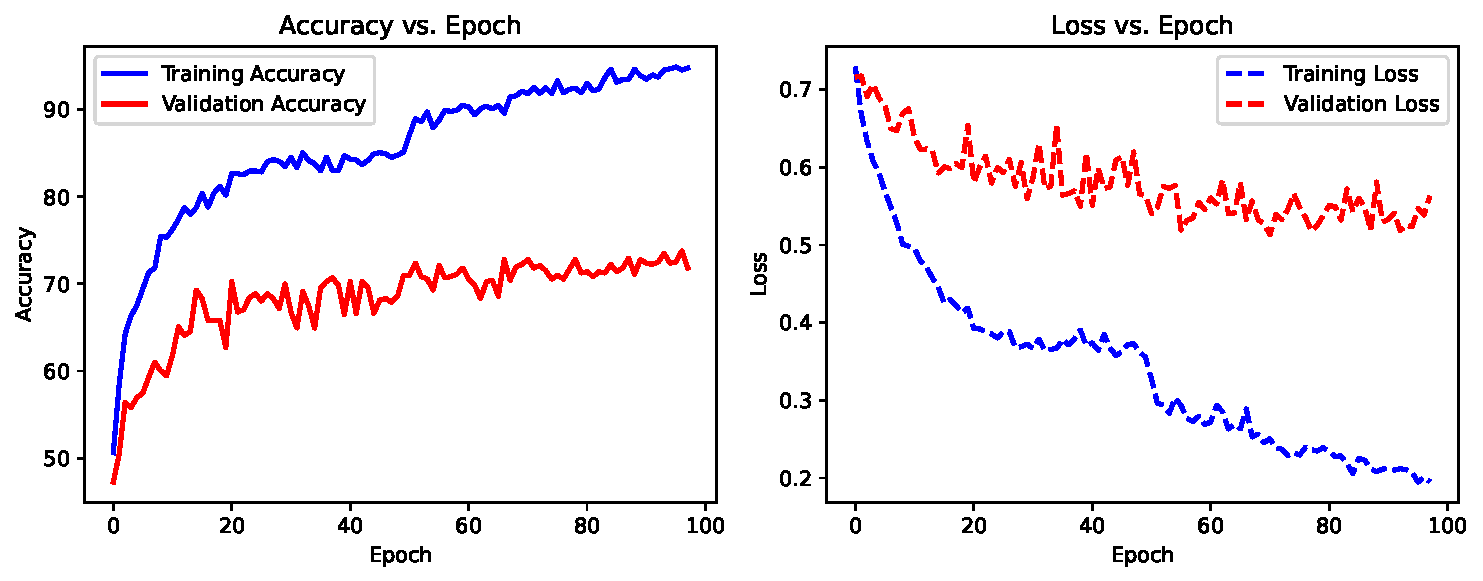
\includegraphics[width=0.45\textwidth]{vis_pdf/TCC_model_perf.pdf}
    \caption{TCC Training (Speaker Dependent - DAIC)}
    \label{fig:training_TCC_daic}
\end{figure}





% \section{Discussion}

% This study's models are designed to predict depression based on classification of PHQ-8 binary scores (???? is it clear), which serve as a binary indicator of depression severity (????). Although the PHQ-8 is a reliable measure of depressive symptoms \cite{phq8}, this reliance raises questions about the necessity and utility of developing machine learning models based on audio data.

% [Add somehow or integrate: maybe there is a faulty self-assessment of depression? However the questions are pretty straight forward, so the chance that somebody doesnt recognizoe these: (include it very briefy )    Little interest or pleasure in doing things         2.  Feeling down, depressed, irritable or hopeless         3.  Trouble falling or staying asleep, or sleeping too much         4.  Feeling tired or having little energy         5.  Poor appetite or overeating         6.  Feeling bad about yourself – or that you are a failure or have let yourself or your family down         7.  Trouble concentrating on things, such as school work, reading or watching television         8.  Moving or speaking so slowly that other people could have noticed? Or the opposite – being so fidgety or restless that you have been moving around a lot more than usual  

% ]

% The technical feasibility of filling out the PHQ-8 survey, which is available online and considered trustworthy, further challenges the practicality of audio-based models. These models might seem redundant when a simpler and well-established method exists. However, audio-based applications could become relevant in scenarios where individuals are reluctant to complete the PHQ-8 survey. This might include cases where individuals, particularly those with severe or major depression, do not seek medical help.

% Nevertheless, the utility of such models is constrained by the limited availability of public datasets, which impacts the robustness and generalizability of the findings. Additionally, factors such as varying audio quality and background noise—dependent on the microphone or the environment—can significantly affect the performance of models trained on audio data. Moreover, feeding the same model with different audio features, such as MFCC or MCC, yields varying results, as revealed in the case of the TCC. This underscores how the choice of audio processing techniques and feature selection can influence model performance, even when the model structure remains the same.

% Furthermore, as highlighted by Bailey \cite{bailey2021gender}, biases such as gender discrepancies within the DAIC-WOZ dataset can lead to performance variations across machine learning models. These biases need to be addressed to enhance the fairness and accuracy of predictive modeling in clinical applications.

% [Add this section as well: 
% The review study listing accuracies but doesnt mention whenever these accuracies are reached on spekear dependent or independent set. Therefore the high numbers are misleading. In reality the high numbers are reached because of the misinterpreatation of the task. What is really happend in speaker dependent approaches is that they separated bunch of people into two groups, and their model recognized whenever an audio sample is from the first group or the second group. But this is not conencted at all to the depression. 
% ]

\section{Discussion}

This study's models are designed to predict depression based on PHQ-8 scores, using them as a binary classifier to distinguish between depressed and non-depressed individuals. While the PHQ-8 is a validated and reliable measure of depressive symptoms \cite{phq8}, this approach raises questions about the necessity of developing audio-based machine learning models.

The PHQ-8 questionnaire assesses clear, observable symptoms including changes in sleep patterns, energy levels, appetite, concentration, and physical activity \cite{phq8qu}. While self-reporting through PHQ-8 is straightforward and accessible online, there may be cases where individuals, particularly those with severe depression, are reluctant to actively seek help or complete surveys. In such scenarios, audio-based detection could provide an alternative screening method.

However, several critical limitations affect the development and deployment of audio-based depression detection models. The scarcity of public datasets constrains model robustness and generalizability. Environmental factors such as audio quality and background noise can significantly impact model performance. Our experiments with the TCC model demonstrated how different audio features (MFCC vs. MCC) yield varying results, highlighting the sensitivity of model performance to feature selection and processing techniques.

A significant methodological concern emerges from my literature review: many studies report high accuracies without clearly distinguishing between speaker-dependent and speaker-independent approaches. This distinction is crucial - speaker-dependent approaches, where audio segments from the same individual appear in both training and testing sets, may artificially inflate accuracy metrics. Such models may be merely recognizing individual speech patterns rather than detecting depression-related characteristics, limiting their real-world applicability.

Additional challenges include dataset biases, such as gender imbalances in the DAIC-WOZ dataset noted by Bailey \cite{bailey2021gender}, which can affect model performance across different demographic groups. These biases need careful consideration when developing models for clinical applications.

The gap between reported accuracies in research and practical clinical utility remains significant. While speaker-dependent approaches report impressive accuracies exceeding 90\%, speaker-independent models - which better reflect real-world scenarios - typically achieve more modest performance. This disparity underscores the importance of rigorous evaluation methodologies that prioritize generalizability over optimistic performance metrics.
%\input{futurework}
\section{Conclusion}
% Summary of contributions and findings
- Start earlier the project next time


\section*{Acknowledgments}  % The asterisk (*) prevents numbering
The author acknowledges the use of ChatGPT and Claude.ai for grammar enhancement in this paper. All technical content, analysis, and conclusions remain the author's original work.

\appendix
%\section{Detailed Feature Descriptions}
%\section{Model Parameters and Configurations}
%\section{Additional Experimental Results}

%\section*{Acknowledgments}
% Thank your advisors, etc.


\clearpage
\printbibliography

% multicolumn version 2
\end{multicols}
\end{document}